\section{Chassis, wedge, forks and side guards}
\label{sec:chassis}

\subsection{Layout and construction}
\label{sec:layout}

The chassis is fully custom and 3D printed in PLA (Figs.~\ref{fig:chassis} to~\ref{fig:dimensions}). The wedge plate and forks form the front of the chassis. The battery holder sits in the front half, with the breadboard carrying the controller, motor driver and sensors beside it. The two gearmotors sit at the rear, each driving a stock sprocket, and the start switch is on the side where the judge can reach it.

% I  wanat to redo this to also point at the slot that allows you to fit a ratcheting socket wrench in to adjust the undriven wheels, and only label a singlne gearmotor. Also we already labeled the wedge elsewhere so I don't want to be redundant.
\begin{figure}[htbp]
  \centering
  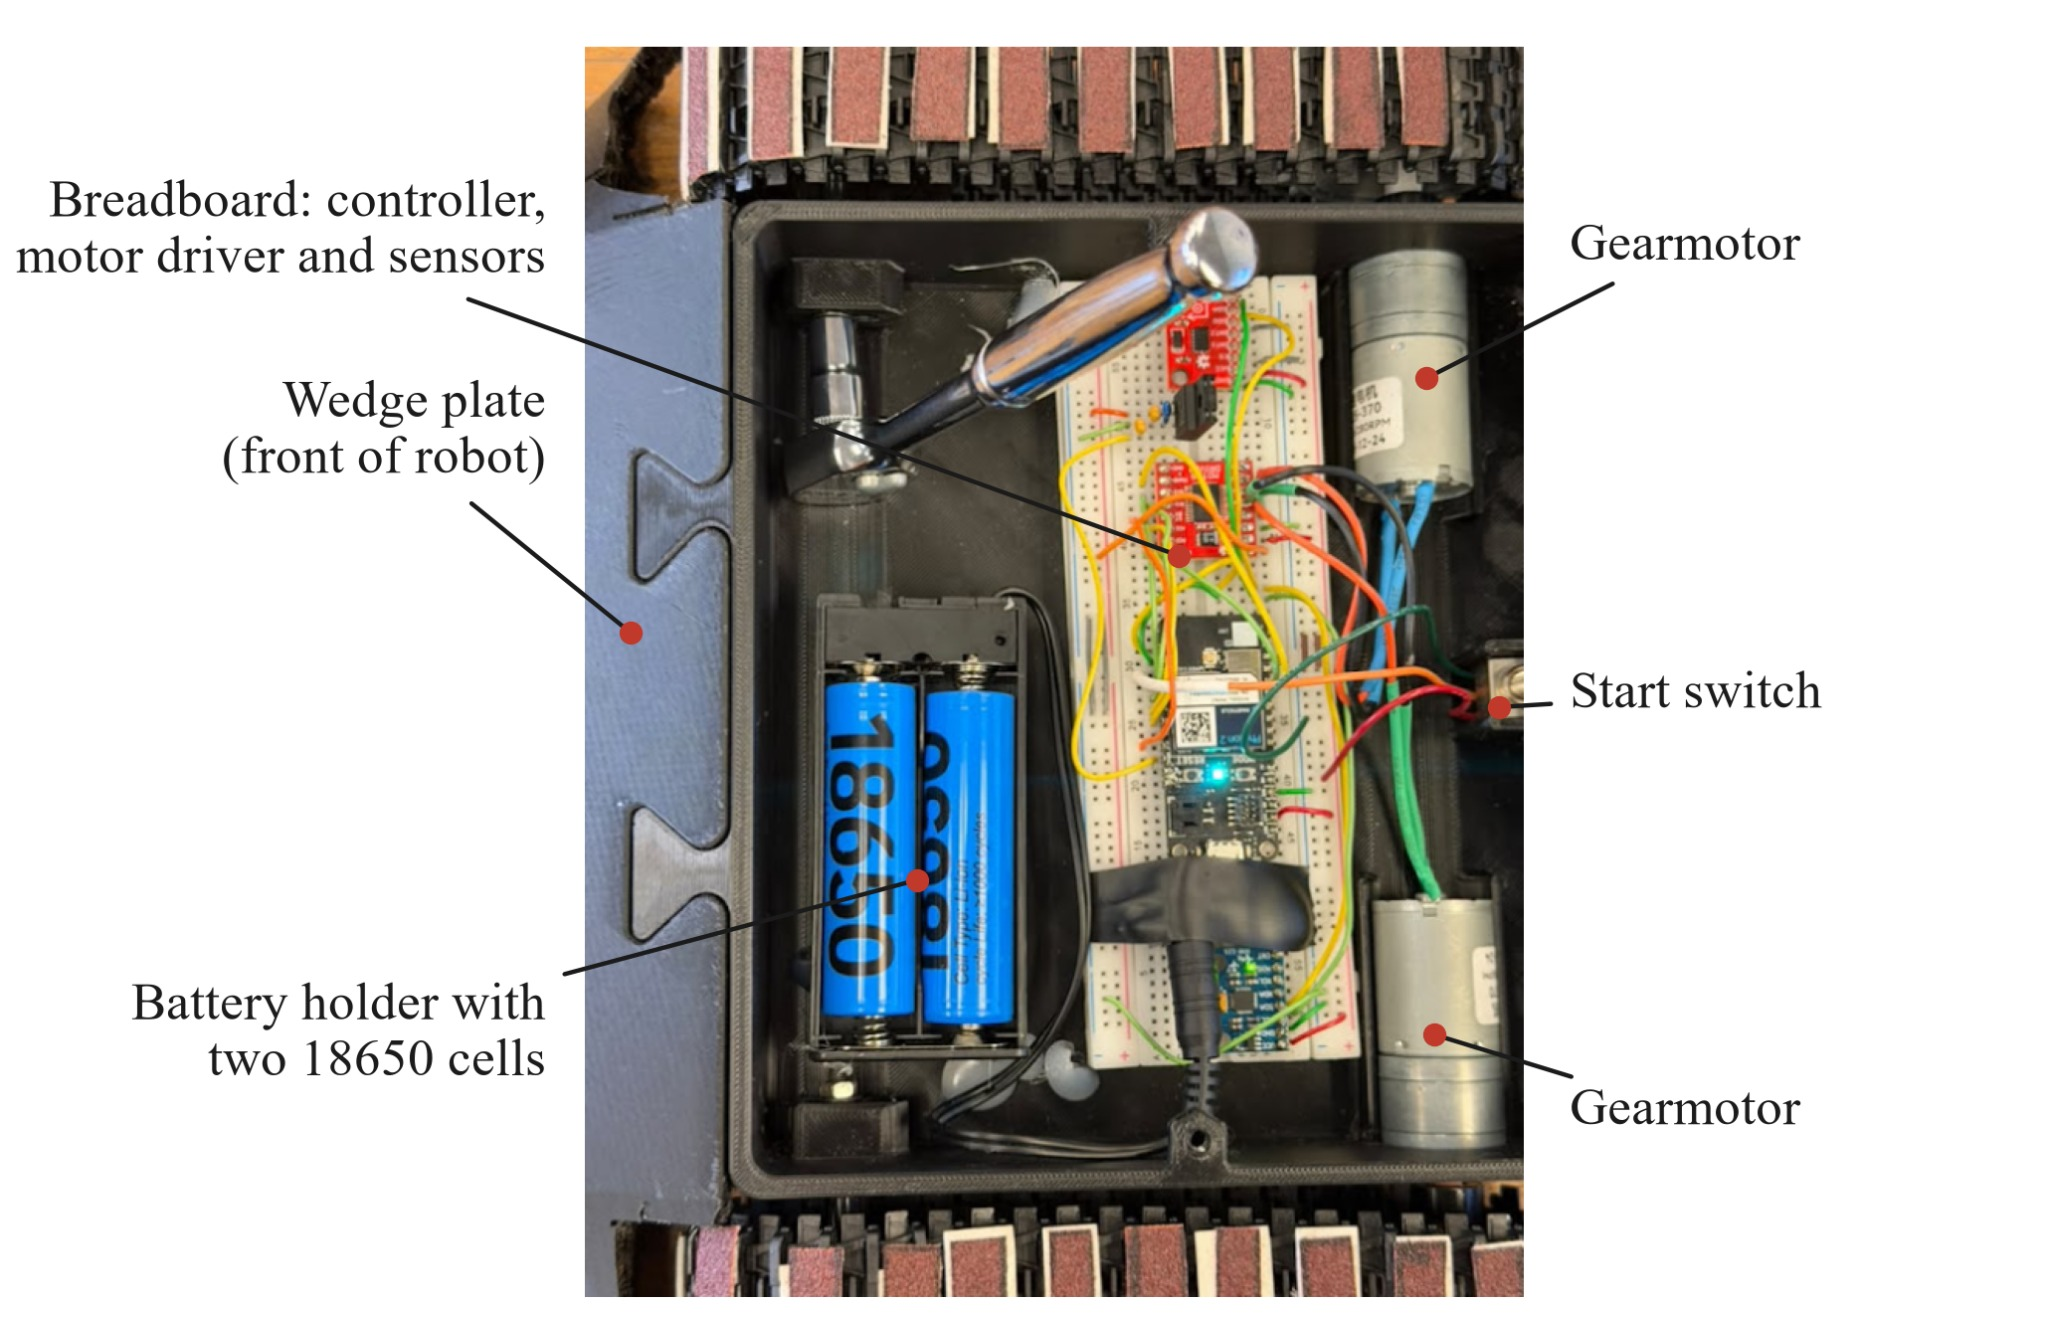
\includegraphics[width=\textwidth]{fig07_chassis.jpg}
  \caption{Inside the chassis with the top plate removed: the wedge plate at the front, the battery holder, the breadboard carrying the controller, motor driver and sensors, the two gearmotors and the start switch.}
  \label{fig:chassis}
\end{figure}

We used a master model workflow where key reference and control geometry flows down through all parts in the assembly. Our final design assembled from four parts: a main body enclosing the electronics, top plate, front wedge, and forks. We ran multiple test prints to check the battery box and board mounting patterns. However, in the final build we hot glued these parts for greater flexibility, which allowed us to change the configuration without reprinting the entire box.

We iterated a few drivetrain mounting prototypes. We realized that sufficient tread tension to prevent the robot from bottoming out on the ridge was crucial. However, to actually assemble then tense the treads would require the wheel pitch to be adjustable. So, we designed slots rather than clearance holes to mount the undriven wheel axle bolts. We also used slicer volume modifiers to raise the infill to 100\% where the bolt applies clamping stress to the plastic, ensuring we could tighten the axles to perfectly rigid with significant tension without the hollow plastic yielding.

Another crucial subassembly was the shaft coupler that adapted the 4mm male D-shaft of the motor to the 6mm female D-shaft of the sprocket. The coupler fits over the motor shaft and inserts into the sprocket shaft recess, fastened to the motor by a shaft collar and to the sprocket by a self-tapping screw that runs through the sprocket.

% if we can use this to guesstimate the positional tolerance of the printer that would be lit and a huge flex, boon to the testing side of thigns.
These required significant measurement, iteration, and testing to function correctly. The fit class between the coupler and each part it connects plays a significant role in how well it functions: too loose a fit (locational clearance) results in a shaft that sits at an angle when tensed with the tread.  It will gyrate and experience particularly particularly unfavorable strain cycles when spun. Too close a fit (interference) means it doesn't assemble. This part requires a running fit. Printing a sweep of different clearance values from 0.05mm to 0.15mm with a resolution of 0.05mm, we found the right clearance for the couplers to be 0.1mm.

Other iteration cycles also centered on clearances and tolerances. Insufficiently clearanced motor mounts and horizontal screw holes resulted in nonfunctional prototypes. After three test iterations, we settled on a mating interface clearance of 0.14mm for the motor mounts and horizontal screw holes.

We followed that up with a few isolated-drivetrain test prints to determine the necessary width for the undriven axle assembly slot such that it assembled easily, which needed to be almost doubled to 15mm from 8mm.

A full prototype chassis followed, then the shaft couplers and motor mounts. To further aid assembly, the top plate included drafted countersunk screw clearance holes and alignment ridges to guide the part into place.

The front wedge we designed as a unified part that wrapped the front of the robot, providing the wedge, side guards, and fork mounts. One difficult thing to design and optimize was the multi-part nature of the robot: manufacturing the entire thing at once wouldn't have been feasible in the build volume of my Prusa Core One+, so it took iteration to find the best places to split and reassemble. Originally, we had planned to print full-length side guards separately, but ditched the idea after realizing that the treads didn't need to be covered along the whole length of the robot. To preempt the need for additional fasteners or gluing, and leave modularity on the table, we designed the front wedge to mate to the rest of the chassis using dovetail joints with semi-permanent snsap fit nubs.
% I have good slicer screenshot for this that I want to include

The front wedge required careful design for printability in order to fit inside the available build volume. For a long, roughly linear part, available volume is maximized by approximately maximizing linear space (the diagonal). Therefore, we included a small 45 degree planar cutoff at the sides to print it at an angle, using tree supports both as supporting outriggers to prevent it from tipping over and to support overhangs.

A significant issue with our design was that the geometry that aimed to fully wrap and enclose the front surface of the treads assumed their nominal pitch of 120mm. However, our assembly procedure was designed to shove the treads as far forward as possible, and we failed to account for this in the design. This resulted in a 5mm interference on all sides between the front surface of the treads and the wedge. Without time to reprint, we used the bandsaw to chop out expanded clearances. This was one contributor to our low drivetrain efficiency, because the side guards were deprived of rigidity and frequently flexed into the treads. (Section~\ref{sec:drivetrain-result}).

At about \qty{4}{in} tall on an \qty{11.75}{in} by \qty{11.4}{in} footprint, the robot cannot tip backward on the \ang{33.4} ramp, and it never came close in testing.

% make this likea "Left: " and "Right: " syntax caption
% also your label for the right is wrong, the right is as a *section view* of the electronics box that cuts away so you can see the internal mounting components better
\begin{figure}[htbp]
  \centering
  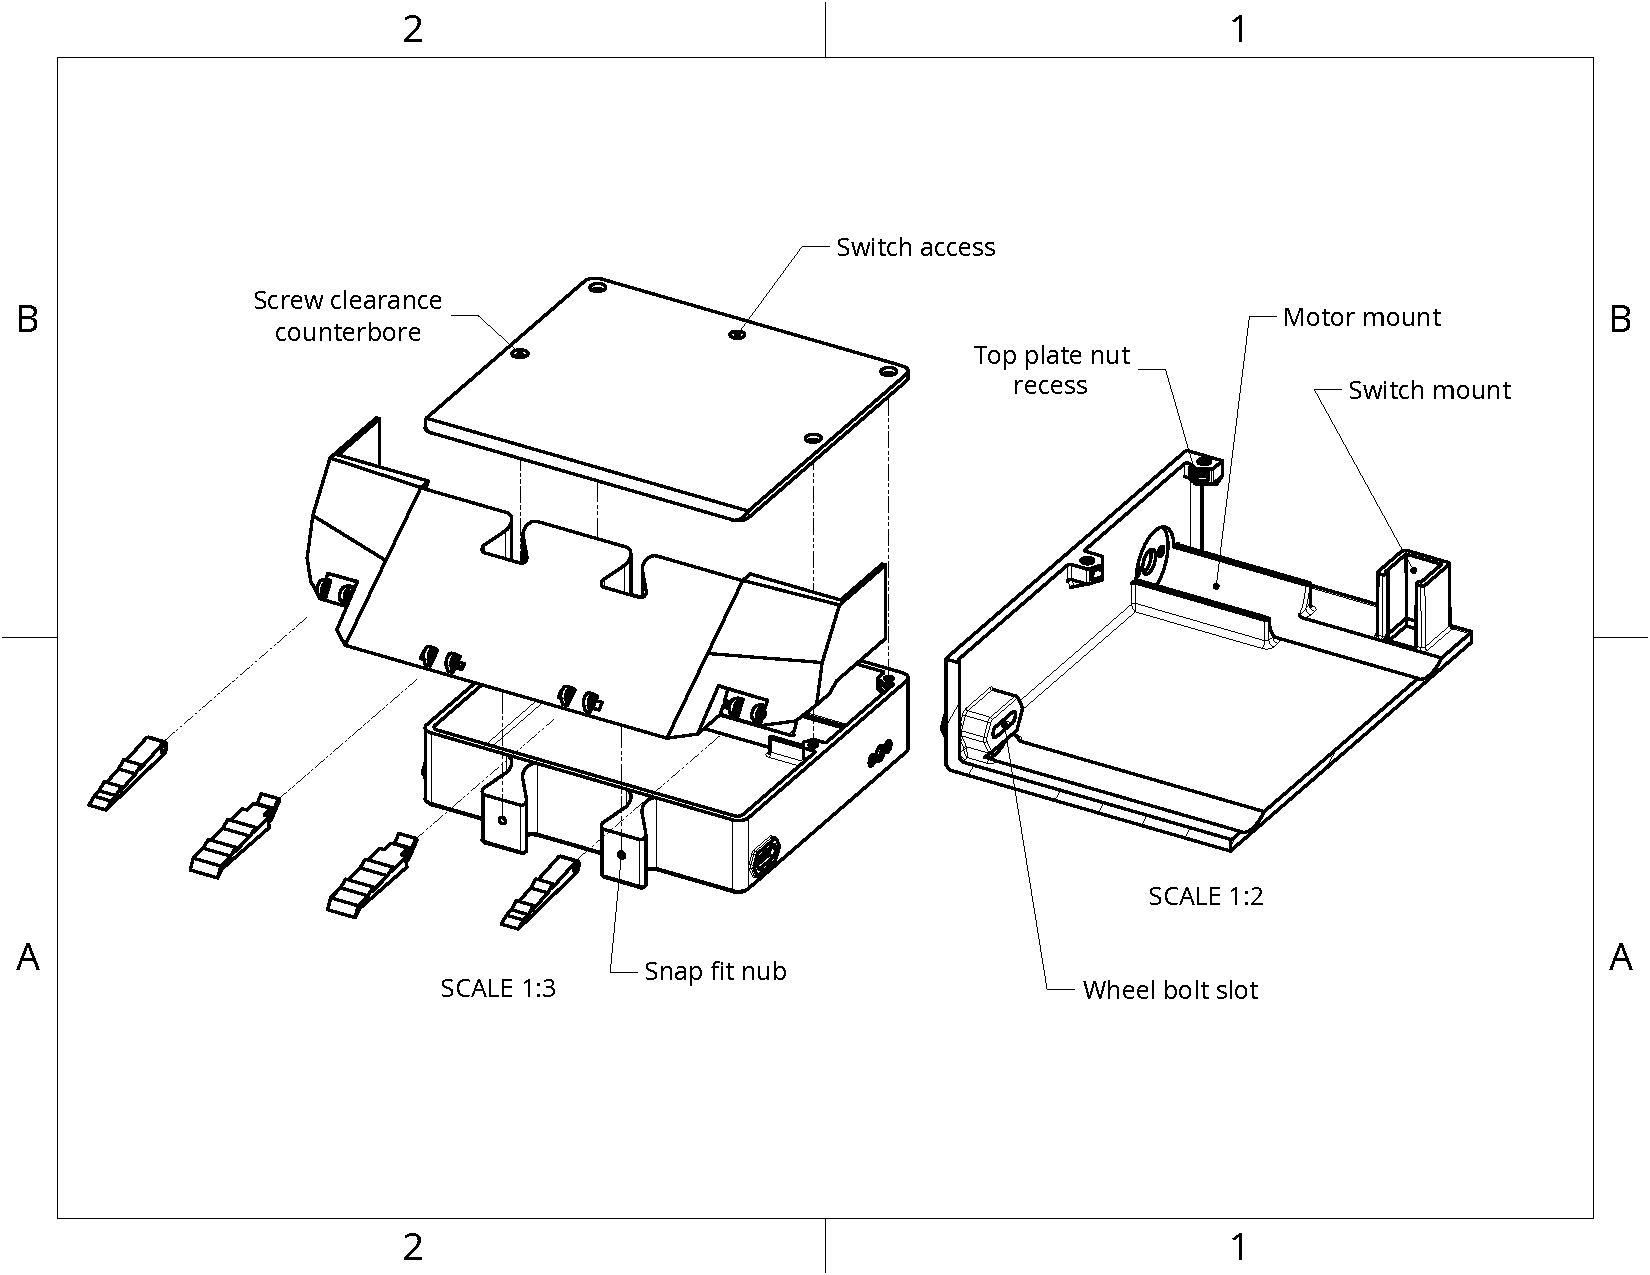
\includegraphics[width=0.8\textwidth]{fig_chassis_assembly.pdf}
  \caption{Exploded assembly drawing of the chassis (scale 1:3), with the base alone at right (scale 1:2).}
  \label{fig:assembly}
\end{figure}

\begin{figure}[htbp]
  \centering
  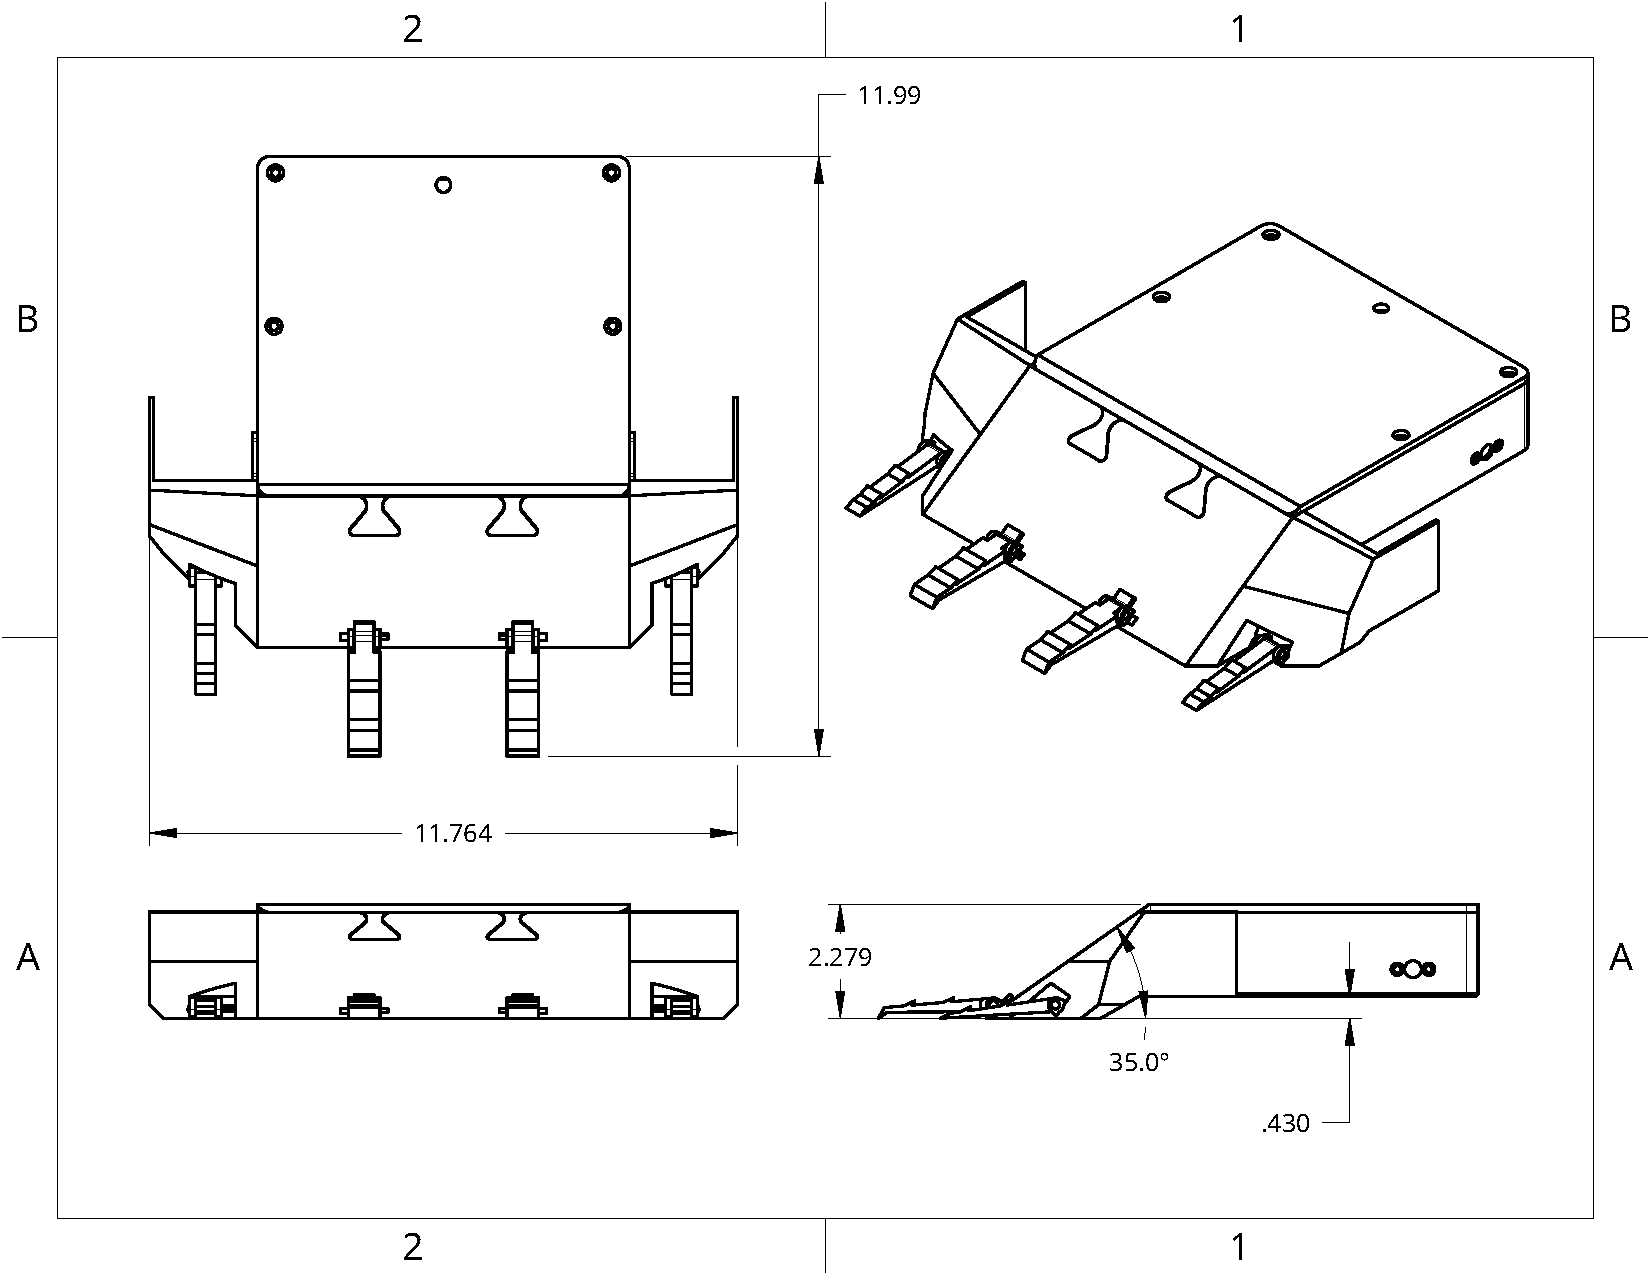
\includegraphics[width=0.8\textwidth]{fig_chassis_dimensions.pdf}
  \caption{Dimensioned drawing of the chassis, in inches. These are the nominal CAD dimensions. Sizes quoted in the text are measured on the built robot and differ from these by print tolerance; the forks and wedge are slightly undersize so they have clearance in their fittings.}
  \label{fig:dimensions}
\end{figure}

\subsection{Wedge and fork geometry}
\label{sec:wedge}

We set the wedge and fork angles from the ramp angle. \tbd{Explain the \mbox{\ang{33}}, \mbox{\ang{57}} and \mbox{\ang{147}} construction from the notebook sketch, what the vulnerability window is, and why the minimum fork angle is \mbox{\ang{33}}.} We left the edge slightly blunt so it would not snap. The forks are shaped to sit flush on the mesa while the tracks are still on the ramp, so the front edge is never raised as the robot arrives (Fig.~\ref{fig:wedge}).

\begin{figure}[htbp]
  \centering
  \placeholderfig{2.2in}{\textbf{\large Figure: drawing here}\\[4pt]Wedge and fork geometry: the \ang{33}, \ang{57} and \ang{147} construction, and the forks sitting flush on the mesa while the tracks are still on the ramp.}
  \caption{\tbd{Drawing of the wedge and fork geometry: the \mbox{\ang{33}}, \mbox{\ang{57}} and \mbox{\ang{147}} construction, and the forks sitting flush on the mesa while the tracks are still on the ramp.}}
  \label{fig:wedge}
\end{figure}

\subsection{Failure Analysis: Shaft couplers}
\label{sec:couplers}

Printed couplers join each motor's \qty{4}{mm} D-shaft to the stock sprocket (Fig.~\ref{fig:coupler}). Each is \qty{25.3}{mm} long and \qty{7.8}{mm} in diameter, round with one flat, and it works as a shaft collar and an adapter at once. The motor shaft fills a \qty{9.3}{mm} deep D-shaped bore at one end and is clamped by a set screw. The outside of the coupler, with its flat, extends the motor's small D-shaft into the larger D-shaped bore of the sprocket, which fits over the first \qty{8}{mm} at the other end, and a self-tapping screw driven into the \qty{1.6}{mm} pilot hole along the axis fastens the sprocket on.

The tracks have to be tight so they do not dip and scrape at the mesa edge. The first couplers, printed standing up, snapped under that tread tension, most of them during assembly rather than in operation. After the contest we treated the coupler as a cantilever and found the largest tread tension it can carry in each print orientation, to see whether orientation explains why those couplers broke and the reprints held.

3D-printed parts are much weaker across their layers than along them, because only the bond between layers resists stress normal to the layer planes. A coupler printed standing up, with its axis along the build direction, carries its bending stress straight across the layer bonds. One printed lying down carries it along the extruded lines (Fig.~\ref{fig:coupler}).

\begin{figure}[htbp]
  \centering
  \placeholderfig{2.2in}{\textbf{\large Figure: drawing here}\\[4pt]Coupler section view from CAD for both print orientations, showing layer direction, shaft bore, sprocket and the load at lever arm $\ell$.}
  \caption{\tbd{Side-by-side slicer views of the coupler printed upright and lying down, with the layer lines visible.}}
  \label{fig:coupler}
\end{figure}

Only one span of the coupler can break. Over its first \qty{8}{mm} it sits inside the rigid sprocket bore, and over its last \qty{9.3}{mm} it wraps the steel motor shaft, which carries the bending there. From 8 to \qty{16}{mm} the plastic carries the load alone.

The tread pulls on the sprocket with a total force $T$, perpendicular to the shaft. Along the free span the bending moment grows toward the motor, so it peaks at the bottom of the motor bore, a distance $\ell$ from the line of the tread. The peak bending stress there is
\begin{equation}
  \sigma = \frac{M c}{I} = \frac{T \ell c}{I}
  \label{eq:bending}
\end{equation}
and the largest pull it can carry before failing is
\begin{equation}
  T_\mathrm{max} = \frac{\sigma_\mathrm{allow}\,(I/c)}{\ell}
  \label{eq:tmax}
\end{equation}
The section at the bottom of the bore is the full D profile with the \qty{1.6}{mm} pilot hole. The coupler turns with the shaft, so the load passes through every direction once per revolution. The worst direction puts the peak stress at a corner of the flat, where $I/c = \qty{36.7}{mm^3}$. The tread runs somewhere on the sprocket's \qty{8}{mm} hub, so $\ell$ lies between 8 and \qty{16}{mm} \tbd{confirm where the tread runs on the hub}.

% no, this is still tread tension - to get the tread *over* and onto the undriven wheel requires significantly more displacement than it just sitting there, you have to force it on even with the slot
Assembly can also bend the coupler with no tread tension at all. A sideways push on the sprocket rim, parallel to the shaft, bends the free span with a lever arm equal to the \qty{25}{mm} sprocket radius, so Eq.~\eqref{eq:tmax} applies with $\ell = \qty{25}{mm}$.

% we didn't use ultimaker PLA and lab tests usually come up with much less optimistic values. Find and use better data.
The two orientations fail in different ways. Printed upright, PLA fractures across its layers without yielding first, so for the upright print $\sigma_\mathrm{allow}$ is its tensile strength at break. Printed flat, it yields first and fractures only after several percent more strain, so the lying print does not snap at its limit: it bends permanently, at its yield strength. Both values come from the Ultimaker PLA data sheet~\cite{ultimaker} \tbd{confirm our filament brand}. Transverse shear is at most \qty{15}{\percent} of the bending stress over this range of $\ell$, and the motor's stall torque of about \qty{0.2}{N.m} adds only about \qty{3}{MPa} of shear, so bending governs.

\begin{table}[htbp]
  \centering
  \caption{Force on the sprocket at which each print orientation fails (upright by fracture, lying by yielding), $T_\mathrm{max}$ from Eq.~\eqref{eq:tmax} with $I/c = \qty{36.7}{mm^3}$.}
  \label{tab:coupler}
  \begin{tabular}{@{}l c c@{}}
    \toprule
    & Upright: stress & Lying: stress \\
    & across the layers & along the layers \\
    \midrule
    $\sigma_\mathrm{allow}$~\cite{ultimaker} (\unit{MPa}) & 33.1, fracture & 52.5, yield (no fracture) \\
    \midrule
    Tread line at the inner edge of the hub, $\ell = \qty{8}{mm}$ & \qty{152}{N} (\qty{34}{\lbf}) & \qty{241}{N} (\qty{54}{\lbf}) \\
    Tread line at mid-hub, $\ell = \qty{12}{mm}$ & \qty{101}{N} (\qty{23}{\lbf}) & \qty{161}{N} (\qty{36}{\lbf}) \\
    Tread line at the outer face, $\ell = \qty{16}{mm}$ & \qty{76}{N} (\qty{17}{\lbf}) & \qty{120}{N} (\qty{27}{\lbf}) \\
    Sideways push on the sprocket rim, $\ell = \qty{25}{mm}$ & \qty{49}{N} (\qty{11}{\lbf}) & \qty{77}{N} (\qty{17}{\lbf}) \\
    \bottomrule
  \end{tabular}
\end{table}

Lying down, the coupler carries 1.6 times the load of the upright print before it fails, and it then bends instead of snapping. We reprinted the couplers lying down and they did not break again.

We never measured the forces during assembly, so Table~\ref{tab:coupler} compares the two orientations rather than predicting when either breaks. Ultimaker's specimens are printed at \qty{100}{\percent} infill with tuned settings, so our couplers were likely weaker than these values \tbd{confirm our print settings}. In operation the coupler is also bent back and forth once per revolution, so it could fail by fatigue below them.
